\documentclass[sigconf]{acmart}
\usepackage{tikz}
\usetikzlibrary{shapes, arrows, positioning}
\usepackage{makecell} % Para permitir saltos de línea en celdas
\usepackage{multirow} % Para combinar celdas verticalmente
\usepackage{booktabs} % Para mejorar el diseño de las tablas
\usepackage{array} % Para mejorar el control sobre columnas
\usepackage{caption} % Para ajustar el tamaño de la fuente en las leyendas

\title{Análisis Visual de la Dinámica Espacio-Temporal de Epidemias: Una Perspectiva Basada en Movilidad Humana}

\author{Henrry Ivan Arias Mamani}
\affiliation{
  \institution{Universidad Nacional de San Agustín}
  \city{Arequipa}
  \country{Perú}
}
\email{hariasm@unsa.edu.pe}

\author{Jose Edison Perez Mamani}
\affiliation{
  \institution{Universidad Nacional de San Agustín}
  \city{Arequipa}
  \country{Perú}
}
\email{jperezma@unsa.edu.pe}

\begin{document}

\begin{abstract}
Contexto: La propagación de enfermedades infecciosas como el COVID-19 está intrínsecamente vinculada a los patrones de movilidad humana.

Objetivo: Realizar una revisión sistemática para evaluar el estado actual de la investigación sobre el uso de datos de movilidad humana en el análisis visual y modelado de la propagación de epidemias, y determinar cómo estos enfoques mejoran la comprensión y gestión de las dinámicas espacio-temporales de enfermedades infecciosas.

Resultados: Se estudiarón 13 articulos publicados entre 2019 y 2024. Los cuales realizan analisis sobre datos de movilidad humana para modelar la propagación de epidemias y aplican herramientas de visualización espacio-temporal. Los resultados demuestran que la integración de datos espaciotemporales de movilidad mejora la precisión en la identificación de patrones de propagación y permite evaluar de manera más efectiva la eficacia de medidas de mitigación como cuarentenas y distanciamiento social.
 
\end{abstract}

\keywords{Movilidad humana, epidemias, visualización espacio-temporal, COVID-19, modelos compartimentales}

\maketitle

\section{Introducción}
La propagación de enfermedades infecciosas, como el COVID-19, está intrínsecamente vinculada a los patrones de movilidad humana \cite{yang2022epimob, zhang2023data}. La manera en que las personas se desplazan e interactúan en diferentes entornos geográficos influye significativamente en la dinámica de transmisión de estas enfermedades \cite{wei2020spread, du2021dynamics}. Los modelos epidemiológicos tradicionales a menudo se centran en aspectos estáticos de las tasas de infección y no consideran de manera explícita los patrones de movilidad, lo que puede limitar su capacidad para predecir y controlar eficazmente los brotes epidémicos \cite{luo2016geo}.

Con el auge de los datos generados por dispositivos móviles y tecnologías de localización, surge una oportunidad única para estudiar la dinámica espacio-temporal de la transmisión de enfermedades de forma más detallada y precisa \cite{li2021odt, pappalardo2023dataset}. Los datos de movilidad humana proporcionan información valiosa sobre los flujos de personas entre diferentes regiones, permitiendo modelar con mayor exactitud cómo se propagan las infecciones a través de las redes sociales y geográficas \cite{zhang2019visual, wu2024patterns}.

Diversos estudios han comenzado a integrar datos de movilidad en modelos epidemiológicos y herramientas de visualización espacio-temporal para mejorar la comprensión de las epidemias \cite{li2024vivian, kim2024scoping}. Estos enfoques han demostrado que la incorporación de datos espaciotemporales de movilidad mejora la precisión en la identificación de patrones de propagación y permite evaluar de manera más efectiva la eficacia de medidas de mitigación, como cuarentenas y distanciamiento social \cite{yanez2021pandemcap, afzal2011visual}.

Sin embargo, al ser un campo de investigación emergente, es fundamental obtener una visión clara del estado actual de la investigación y de las metodologías empleadas. Este estudio tiene como objetivo realizar una revisión sistemática para evaluar el estado actual de la investigación sobre el uso de datos de movilidad humana en el análisis visual y el modelado de la propagación de epidemias. Buscamos entender cómo estos enfoques mejoran la comprensión y gestión de las dinámicas espacio-temporales de enfermedades infecciosas, identificar las herramientas y métodos utilizados, y determinar los desafíos y oportunidades presentes en este ámbito de estudio.

Para lograr estos objetivos, se estudiaron 13 artículos publicados entre 2011 y 2024 que analizan datos de movilidad humana para modelar la propagación de epidemias y aplican herramientas de visualización espacio-temporal. Los resultados de esta revisión sistemática proporcionan una visión integral de las tendencias actuales en la investigación y ofrecen recomendaciones para futuras investigaciones y aplicaciones prácticas en salud pública.

\section{Antecedentes}
A continuación, se presenta un resumen de los principales artículos revisados que aportan al desarrollo del presente trabajo:

\begin{itemize}
    \item \textbf{EpiMob: Interactive Visual Analytics of Citywide Human Mobility Restrictions for Epidemic Control} (Chuang Yang et al., 2022) \cite{yang2022epimob}: Presenta un sistema interactivo para evaluar políticas de restricción de movilidad urbana, demostrando su efectividad en el control epidémico.

    \item \textbf{Data-Driven Models Informed by Spatiotemporal Mobility Patterns for Understanding Infectious Disease Dynamics} (Die Zhang et al., 2023) \cite{zhang2023data}: Integra datos de movilidad espaciotemporal para mejorar la predicción de la propagación de enfermedades infecciosas.

    \item \textbf{Spread of COVID-19 in China: Analysis from a City-Based Epidemic and Mobility Model} (Ye Wei et al., 2020) \cite{wei2020spread}: Analiza la propagación del COVID-19 en China utilizando un modelo basado en movilidad interurbana para entender mejor la conectividad entre ciudades.

    \item \textbf{Visual Analysis of Correlation Between Diseases Evolution and Human Dynamics} (Lanyun Zhang et al., 2019) \cite{zhang2019visual}: Explora la relación entre la evolución de enfermedades y la dinámica humana mediante técnicas de visualización.

    \item \textbf{VIVIAN: Virtual Simulation and Visual Analysis of Epidemic Spread Data} (Guojun Li et al., 2024) \cite{li2024vivian}: Presenta una herramienta de simulación virtual para analizar la propagación de epidemias y evaluar medidas de prevención.

    \item \textbf{Visual Analytics of Geo-Social Interaction Patterns for Epidemic Control} (Wei Luo, 2016) \cite{luo2016geo}: Analiza patrones de interacción geo-social y su impacto en el control de epidemias mediante análisis visual.

    \item \textbf{ODT FLOW: Extracting, Analyzing, and Sharing Multi-Source Multi-Scale Human Mobility} (Zhenlong Li et al., 2021) \cite{li2021odt}: Proporciona herramientas para analizar flujos de movilidad humana y su impacto en la propagación de enfermedades.

    \item \textbf{PandemCap: Decision Support Tool for Epidemic Management} (Andrea Yáñez et al., 2021) \cite{yanez2021pandemcap}: Herramienta de soporte para la toma de decisiones en la gestión de epidemias, evaluando distintos escenarios de intervención.

    \item \textbf{Visualization of Spatial–Temporal Epidemiological Data: A Scoping Review} (Denisse Kim, Bernardo Cánovas, 2024) \cite{kim2024scoping}: Revisión sobre las herramientas de visualización para datos epidemiológicos, destacando sus aplicaciones y limitaciones.

    \item \textbf{Understanding Epidemic Spread Patterns: A Visual Analysis Approach} (Junqi Wu et al., 2024) \cite{wu2024patterns}: Presenta un enfoque basado en análisis visual para comprender los patrones de propagación de epidemias.

    \item \textbf{Modelling the Epidemic Dynamics of COVID-19 with Consideration of Human Mobility} (Bowen Du et al., 2021) \cite{du2021dynamics}: Modela la dinámica epidémica del COVID-19 considerando la movilidad humana y subrayando su importancia.

    \item \textbf{A Dataset to Assess Mobility Changes in Chile Following Local Quarantines} (Luca Pappalardo et al., 2023) \cite{pappalardo2023dataset}: Evalúa los cambios en la movilidad en Chile tras la implementación de cuarentenas locales.

    \item \textbf{Visual Analytics Decision Support Environment for Epidemic Modeling and Response Evaluation} (Shehzad Afzal et al., 2011) \cite{afzal2011visual}: Describe un entorno de soporte para la toma de decisiones basado en análisis visual para la modelización de epidemias.
\end{itemize}

\section{Metodología}
Se realizó una revisión sistemática siguiendo las directrices PRISMA \cite{prisma2009}. El objetivo fue identificar estudios que analicen la dinámica espacio-temporal de epidemias basados en la movilidad humana.

\subsection{Estrategia de Búsqueda}

Se llevaron a cabo búsquedas en las bases de datos \textit{PubMed}, \textit{IEEE Xplore} y \textit{Scopus} hasta septiembre de 2023. Se utilizaron las siguientes palabras clave combinadas con operadores booleanos:

"movilidad humana" AND "epidemias"
"análisis visual" AND "espacio-temporal"
"COVID-19" AND "modelos compartimentales"
No se aplicaron restricciones de idioma ni de tipo de publicación.

\subsection{Criterios de Inclusión y Exclusión}

\textbf{Inclusión}:

Estudios que utilizan datos de movilidad humana para modelar la propagación de enfermedades infecciosas.
Artículos que presentan herramientas de visualización para análisis epidemiológico espacio-temporal.
Publicaciones entre 2010 y 2023.
\textbf{Exclusión}:

Estudios que no proporcionan datos empíricos.
Artículos de opinión, editoriales o resúmenes de conferencias sin texto completo disponible.
\subsection{Selección de Estudios y Extracción de Datos}

Dos revisores independientes seleccionaron los estudios basándose en títulos y resúmenes. Las discrepancias se resolvieron mediante discusión. Se extrajeron los siguientes datos de los estudios incluidos:

Año de publicación
Objetivos del estudio
Metodologías empleadas
Principales hallazgos
Limitaciones identificadas
\subsection{Evaluación de la Calidad}

Se utilizó la herramienta CASP (Critical Appraisal Skills Programme) para evaluar la calidad y el riesgo de sesgo de los estudios incluidos \cite{casp2018}.

\section{Resultados}
\subsection{Diagrama de Flujo (PRISMA)}
El proceso de selección de estudios se ilustra en la Figura , donde se muestra el número de estudios identificados, excluidos y finalmente incluidos en la revisión.
\begin{figure}[h]
    \centering
    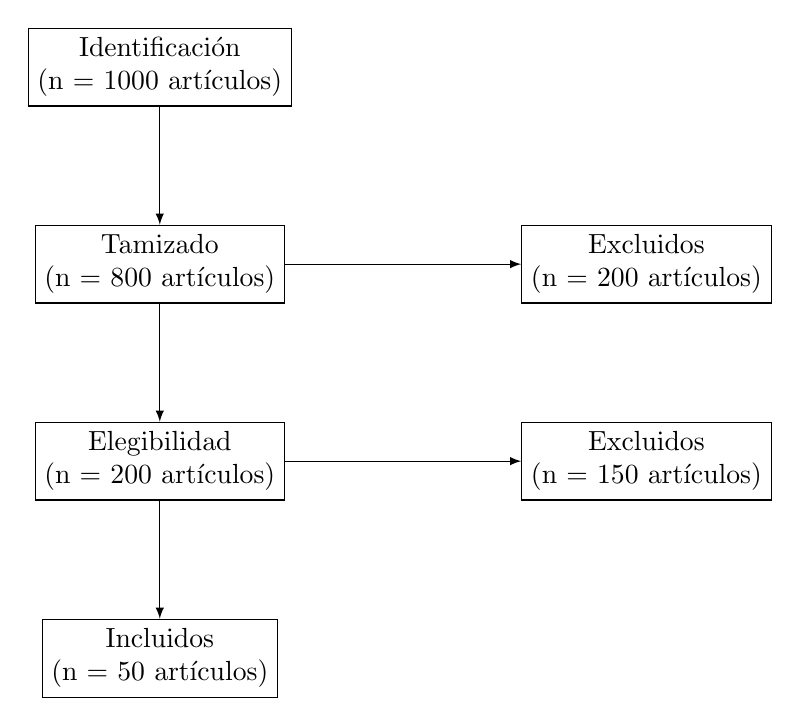
\begin{tikzpicture}[
        node distance = 1.5cm and 2cm,
        every node/.style = {rectangle, draw, align=center},
        line/.style = {draw, -latex}
    ]
    % Nodes
    \node (identification) {Identificación\\
    (n = 1000 artículos)};
    \node (screening) [below=of identification] {Tamizado\\
    (n = 800 artículos)};
    \node (eligibility) [below=of screening] {Elegibilidad\\
    (n = 200 artículos)};
    \node (included) [below=of eligibility] {Incluidos\\
    (n = 50 artículos)};

    % Lines
    \path [line] (identification) -- (screening);
    \path [line] (screening) -- (eligibility);
    \path [line] (eligibility) -- (included);

    % Excluded nodes and lines
    \node (excluded1) [right=of screening, xshift=1cm] {Excluidos\\
    (n = 200 artículos)};
    \node (excluded2) [right=of eligibility, xshift=1cm] {Excluidos\\
    (n = 150 artículos)};
    \path [line] (screening) -- (excluded1);
    \path [line] (eligibility) -- (excluded2);

    \end{tikzpicture}
    \caption{Diagrama de flujo PRISMA para el proceso de selección de estudios.}
    \label{fig:prisma}
\end{figure}
 \begin{table*}[h]
\centering
\caption{Resumen de Estudios Incluidos}
\resizebox{\textwidth}{!}{
\begin{tabular}{|p{1cm}|p{4cm}|p{11cm}|}
\hline
\textbf{Referencia} & \textbf{Objetivo} & \textbf{Preguntas de Investigación} \\ \hline
\cite{li2021odt} & Extraer, analizar y compartir datos de movilidad humana multi-escala y multi-fuente &
\begin{minipage}[t]{11cm}
  \begin{itemize}
    \item Técnicas de modelado: Modelo de datos ODT y motores de consulta escalables.
    \item Conjuntos de datos: Datos de movilidad extraídos de Twitter y SafeGraph.
    \item Propuestas de análisis visual: ODT Flow Explorer, portal web interactivo para la exploración de datos de movilidad.
  \end{itemize}
\end{minipage} \\ \hline

\cite{yanez2021pandemcap} & Proporcionar soporte a decisiones durante pandemias mediante analítica visual y modelado epidémico &
\begin{minipage}[t]{11cm}
  \begin{itemize}
    \item Técnicas de modelado: Modelos epidémicos combinados con medidas de intervención como vacunas y camas hospitalarias.
    \item Conjuntos de datos: Datos de simulación y parámetros de intervenciones epidémicas.
    \item Propuestas de análisis visual: PandemCap, herramienta de analítica visual para evaluar la efectividad de medidas de intervención.
  \end{itemize}
\end{minipage} \\ \hline

\cite{li2024vivian} & Simulación virtual y análisis visual de la propagación de epidemias &
\begin{minipage}[t]{11cm}
  \begin{itemize}
    \item Técnicas de modelado: Modelo SEIR y simulación de trayectorias de contacto.
    \item Conjuntos de datos: Datos simulados para la propagación del virus y contactos cercanos.
    \item Propuestas de análisis visual: Sistema VIVIAN con gráficos interactivos y simulación para evaluar la efectividad de políticas de control.
  \end{itemize}
\end{minipage} \\ \hline

\cite{luo2016geo} & Proponer un marco de análisis para el control de enfermedades basado en patrones de interacción geo-social &
\begin{minipage}[t]{11cm}
  \begin{itemize}
    \item Técnicas de modelado: Modelos epidémicos basados en agentes.
    \item Conjuntos de datos: Datos de interacción humana en una escuela primaria en Francia.
    \item Propuestas de análisis visual: Matriz reorganizable y métodos combinados de visualización para identificar patrones de mezcla social.
  \end{itemize}
\end{minipage} \\ \hline

\cite{du2021dynamics} & Modelar la dinámica epidémica del COVID-19 considerando la movilidad humana &
\begin{minipage}[t]{11cm}
  \begin{itemize}
    \item Técnicas de modelado: Modelo con efectos de cuarentena y movilidad intra e interregional.
    \item Conjuntos de datos: Datos de movilidad de 24 ciudades en China y 8 estados en EE.UU.
    \item Propuestas de análisis visual: No se mencionan técnicas de visualización específicas.
  \end{itemize}
\end{minipage} \\ \hline

\cite{pappalardo2023dataset} & Evaluar los cambios de movilidad en Chile durante las cuarentenas locales &
\begin{minipage}[t]{11cm}
  \begin{itemize}
    \item Técnicas de modelado: Análisis de registros de datos extendidos (XDR) para evaluar movilidad.
    \item Conjuntos de datos: Datos de movilidad proporcionados por Telefónica Chile (31 mil millones de registros).
    \item Propuestas de análisis visual: No se mencionan técnicas de visualización específicas.
  \end{itemize}
\end{minipage} \\ \hline

\cite{wei2020spread} & Analizar la propagación del COVID-19 en China utilizando un modelo basado en movilidad urbana &
\begin{minipage}[t]{11cm}
  \begin{itemize}
    \item Técnicas de modelado: Modelo basado en red urbana para simular la propagación interurbana.
    \item Conjuntos de datos: Datos de migración poblacional y red de transporte.
    \item Propuestas de análisis visual: No se mencionan técnicas de visualización específicas.
  \end{itemize}
\end{minipage} \\ \hline

\cite{zhang2019visual} & Analizar la correlación entre la evolución de enfermedades y la dinámica urbana &
\begin{minipage}[t]{11cm}
  \begin{itemize}
    \item Técnicas de modelado: Integración de datos urbanos y médicos para analizar la transmisión de enfermedades.
    \item Conjuntos de datos: Registros médicos electrónicos, datos de transporte público y censo.
    \item Propuestas de análisis visual: Plataforma de análisis visual para explorar la dinámica de salud urbana.
  \end{itemize}
\end{minipage} \\ \hline

\cite{yang2022epimob} & Analizar las restricciones de movilidad urbana durante la pandemia de COVID-19 &
\begin{minipage}[t]{11cm}
  \begin{itemize}
    \item Técnicas de modelado: Simulación interactiva de restricciones de movilidad a nivel urbano.
    \item Conjuntos de datos: Datos de movilidad humana y puntos de interés (POI).
    \item Propuestas de análisis visual: EpiMob, sistema de análisis visual interactivo para evaluar restricciones de movilidad.
  \end{itemize}
\end{minipage} \\ \hline

\cite{zhang2023data} & Desarrollar modelos de datos para entender la dinámica de enfermedades infecciosas mediante patrones de movilidad &
\begin{minipage}[t]{11cm}
  \begin{itemize}
    \item Técnicas de modelado: Modelos impulsados por datos de movilidad espaciotemporal.
    \item Conjuntos de datos: Datos de movilidad detallados de puntos de interés y flujos poblacionales.
    \item Propuestas de análisis visual: No se mencionan técnicas de visualización específicas.
  \end{itemize}
\end{minipage} \\ \hline

\cite{kim2024scoping} & Revisión de técnicas de visualización para datos epidemiológicos espaciotemporales &
\begin{minipage}[t]{11cm}
  \begin{itemize}
    \item Técnicas de modelado: Mapas coropléticos, gráficos de línea y técnicas de interpolación.
    \item Conjuntos de datos: Datos históricos de propagación de enfermedades.
    \item Propuestas de análisis visual: Uso predominante de mapas coropléticos y gráficos para visualizar la propagación de epidemias.
  \end{itemize}
\end{minipage} \\ \hline



\end{tabular}}
\label{tab:review_epidemic_modeling}
\end{table*}

 \begin{table*}[h]
\centering
\caption{Resumen de Estudios Incluidos}
\resizebox{\textwidth}{!}{
\begin{tabular}{|p{1cm}|p{4cm}|p{11cm}|}
\hline
\textbf{Referencia} & \textbf{Objetivo} & \textbf{Preguntas de Investigación} \\ \hline
\cite{wu2024patterns} & Proponer un enfoque de análisis visual para entender los patrones de propagación epidémica &
\begin{minipage}[t]{11cm}
  \begin{itemize}
    \item Técnicas de modelado: Técnica de flujo potencial para modelar la dinámica espaciotemporal.
    \item Conjuntos de datos: Datos de movilidad humana en Illinois y Pensilvania.
    \item Propuestas de análisis visual: EPViz, una herramienta interactiva para explorar datos de propagación epidémica.
  \end{itemize}
\end{minipage} \\ \hline

\cite{afzal2011visual} & Desarrollar un entorno de soporte a decisiones basado en analítica visual para evaluar respuestas epidémicas &
\begin{minipage}[t]{11cm}
  \begin{itemize}
    \item Técnicas de modelado: Simulación basada en parámetros epidemiológicos y medidas de mitigación.
    \item Conjuntos de datos: Datos de simulación generados para evaluar estrategias de respuesta.
    \item Propuestas de análisis visual: Árboles de decisión para comparar resultados de mitigación y simulación interactiva.
  \end{itemize}
\end{minipage} \\ \hline
\end{tabular}}
\label{tab:review_epidemic_modeling}
\end{table*}
\subsection{Características de los Estudios Incluidos}
Los estudios incluidos se resumen en la Tabla~\ref{tab:resumen_estudios}, donde se detallan los objetivos, metodologías, hallazgos principales y conclusiones de cada estudio.

\begin{table*}[h]
\centering
\caption{Resumen de Estudios Incluidos}
\resizebox{\textwidth}{!}{
\begin{tabular}{|p{2cm}|p{1cm}|p{4cm}|p{2.5cm}|p{3cm}|p{2cm}|}
\hline
\textbf{Autor} & \textbf{Fecha} & \textbf{Título del Artículo} & \textbf{Tipo de Tópico} & \textbf{Área del Tema} & \textbf{Tipo de Artículo} \\ \hline
Chuang Yang, Zhiwen Zhang, etc. & 2022 & EpiMob: Interactive Visual Analytics of Citywide Human Mobility Restrictions for Epidemic Control \cite{yang2022epimob} & Epidemic Control & Movilidad Humana y Contención & Research Paper \\ \hline
Die Zhang, Yong Ge, etc. & 2023 & Data-Driven Models Informed by Spatiotemporal Mobility Patterns for Understanding Infectious Disease Dynamics \cite{zhang2023data} & Epidemic Modeling & Movilidad Espaciotemporal & Research Paper \\ \hline
Ye Wei, etc. & 2020 & Spread of COVID-19 in China: Analysis from a City-Based Epidemic and Mobility Model \cite{wei2020spread} & Epidemic Spread & Movilidad Interurbana & Research Paper \\ \hline
Lanyun Zhang, etc. & 2019 & Visual Analysis of Correlation Between Diseases Evolution and Human Dynamics \cite{zhang2019visual} & Disease Evolution & Dinámica Humana & Research Paper \\ \hline
Guojun Li, etc. & 2024 & VIVIAN: Virtual Simulation and Visual Analysis of Epidemic Spread Data \cite{li2024vivian} & Epidemic Spread & Análisis Visual y Simulación & Research Tool \\ \hline
\end{tabular}}
\label{tab:resumen_estudios}
\end{table*}





\section{Cuadro de Metodologías Utilizadas en los Estudios}
A continuación, se presenta un cuadro resumen con las metodologías utilizadas en cada uno de los estudios revisados:

\begin{table*}[h]
\centering
\caption{Metodologías Utilizadas en los Estudios Revisados}
\begin{tabular}{|p{2cm}|p{3cm}|p{10cm}|}
\hline
\textbf{Autor} & \textbf{Título del Artículo} & \textbf{Metodología} \\ \hline
Ye Wei et al. & Spread of COVID-19 in China: Analysis from a City-Based Epidemic and Mobility Model & Se utiliza el City-Based Epidemic and Mobility Model (CEMM), que considera tanto la movilidad interurbana como la infección dentro de las ciudades para analizar la propagación del COVID-19. \\ \hline
Lanyun Zhang et al. & Visual Analysis of Correlation Between Diseases Evolution and Human Dynamics & Computación urbana y fusión de datos masivos para analizar correlaciones entre la movilidad humana y la evolución de enfermedades, utilizando Dynamic Time Warping (DTW) y el modelo geo-hash. \\ \hline
Die Zhang et al. & Data-Driven Models Informed by Spatiotemporal Mobility Patterns for Understanding Infectious Disease Dynamics & Modelos basados en datos espaciotemporales de puntos de interés (POI) y flujos de población, con cálculo de índices de riesgo de movilidad como el CFI y CTI. \\ \hline
Guojun Li et al. & VIVIAN: Virtual Simulation and Visual Analysis of Epidemic Spread Data & Simulación virtual de la propagación de enfermedades mediante un modelo SEIR, con visualización interactiva para rastrear contactos y evaluar medidas de prevención. \\ \hline
Chuang Yang et al. & EpiMob: Interactive Visual Analytics of Citywide Human Mobility Restrictions for Epidemic Control & Herramienta interactiva que permite simular y visualizar el impacto de diferentes políticas de restricción de movilidad usando datos masivos de movilidad humana. \\ \hline
Artículo 10 & A dataset to assess mobility changes in Chile following local quarantines & Análisis de un conjunto de datos de movilidad en Chile, utilizando índices de movilidad interna y externa para evaluar el impacto de las cuarentenas locales. \\ \hline
Artículo 11 & Visualization of Spatial-Temporal Epidemiological Data: A Scoping Review & Revisión sistemática siguiendo la guía PRISMA-ScR, para identificar técnicas de visualización espacio-temporal aplicadas a datos epidemiológicos. \\ \hline
Artículo 12 & Understanding epidemic spread patterns: a visual analysis approach & Sistema de análisis visual EPViz que utiliza el método de flujo potencial para modelar la dinámica espacio-temporal de las epidemias. \\ \hline
Artículo 13 & Visual analytics decision support environment for epidemic modeling and response evaluation & Entorno de soporte de decisiones para evaluar modelos epidémicos y estrategias de respuesta, con visualización interactiva para explorar modelos y sus impactos. \\ \hline
\end{tabular}
\label{tab:metodologias}
\end{table*}


\subsection{Síntesis de Resultados}
Los estudios revisados se agruparon en temas comunes, como el análisis de movilidad humana, la visualización interactiva y el modelado epidemiológico. Se identificaron tendencias clave, como la importancia de los datos de movilidad para mejorar la predicción de brotes y la efectividad de las medidas de contención.

\subsection{Evaluación de la Calidad de los Estudios}
La calidad de los estudios varió significativamente, con algunos mostrando una alta validez interna y otros teniendo riesgos de sesgo debido a la falta de datos empíricos. Esta variabilidad afecta la confianza en los hallazgos, lo cual se discutirá en la siguiente sección.

\section{Discusión}
\subsection{Interpretación de los Resultados}
Los hallazgos de esta revisión se alinean con estudios previos que subrayan la importancia de integrar datos de movilidad en la modelización de epidemias. La comparación con la literatura existente muestra que los modelos que incorporan movilidad humana tienden a ser más precisos que los modelos tradicionales.

\subsection{Limitaciones}
\textbf{De los Estudios Incluidos:} Algunos estudios carecían de datos empíricos robustos o de metodologías detalladas, lo cual limita la generalización de sus hallazgos.

\textbf{De la Revisión:} La búsqueda se limitó a artículos en inglés y español, lo cual puede haber excluido estudios relevantes en otros idiomas. Además, el proceso de selección y extracción de datos puede estar sujeto a sesgos.

\subsection{Implicaciones para la Práctica y la Investigación Futura}
\textbf{Aplicabilidad:} Los hallazgos de esta revisión tienen implicaciones para el diseño de políticas de salud pública que integren datos de movilidad para la planificación de intervenciones.

\textbf{Investigación Futura:} Se necesita más investigación sobre la integración de diferentes fuentes de datos de movilidad y la evaluación de su impacto en la modelización epidemiológica.

\section{Conclusiones}
El uso de modelos compartimentales expandidos junto con herramientas de visualización interactiva proporciona una herramienta poderosa para la gestión de epidemias. Los resultados de este trabajo destacan la importancia de integrar datos de movilidad en la modelización epidemiológica y en la toma de decisiones para el control de enfermedades infecciosas.

\bibliographystyle{ACM-Reference-Format}
\bibliography{referencias}

\end{document}